\documentclass[a4paper, 12pt]{article}

\title{\tikzlogo 代码查阅手册}
\author{张梦磊}
\date{2017 年 11 月 12 日}
\pagenumbering{gobble} % 不显示页码


\usepackage[left=1cm, right=1cm, top=1.5cm, bottom=1.5cm]{geometry}
\usepackage{ctex}
\usepackage{tikz}
\usetikzlibrary{math,positioning,arrows,calc,shapes}

\graphicspath{{Source/}{Source/Figures/}}

\pgfdeclarelayer{secbackground}
\pgfdeclarelayer{background}
\pgfdeclarelayer{foreground}
\pgfsetlayers{secbackground,background,main,foreground}

\usepackage{pgfkeys}
\usepackage{tcolorbox}
\tcbuselibrary{documentation,minted}
\tcbset{listing engine=minted}

\usepackage{esvect} % shape.tex 例子中画向量需要 \vv
\usepackage{bm}
\usepackage{amsmath}
\usepackage{fontspec}
\setmonofont{Source Code Pro}

\definecolor{papercolor}{RGB}{255, 236, 229}
\pagecolor{papercolor}

\usepackage{xspace}
\newcommand{\tikzlogo}{Ti\textcolor{orange}{\emph{k}}Z\xspace}
\newcommand{\pgflogo}{\textsc{PGF}\xspace}

% 定义缩写, 第三个空为选项, \lxcode|...| 输入行间代码
\newmintinline[lxcode]{latex}{}

\tcbset{%
	docexample/.style={colframe=gray!40!white,colback=ExampleBack,
		before skip=\medskipamount,after skip=\medskipamount,
		fontlower=\footnotesize, documentation minted options={fontsize=\zihao{-5}},}%
}

\begin{document}
\maketitle
\begin{minipage}{.9\textwidth}
\centerline{前言}
本手册准备收集自己平时写过的 \tikzlogo 代码, 主要将其中可以复用的代码提炼出来, 方便日后使用. 要正常编译所有代码, 使用:

\begin{minted}{latex}
\usepackage{tikz}
\usetikzlibrary{math,positioning,arrows,calc,shapes}
% 下面可以不需要, 但某些代码要
\usepackage{esvect} % shape.tex 例子中画向量需要 \vv
\usepackage{bm}
\usepackage{amsmath}
\end{minted}
\end{minipage}
\tableofcontents
\section{导言区 -- Preamble}
\subsection{图像较简单的情况}

\begin{minted}{latex}
	
\documentclass{article}

\usepackage{ctex}
\usepackage{tikz}
\usetikzlibrary{arrows, positioning,calc}

\usepackage[active, tightpage]{preview}
\PreviewEnvironment{tikzpicture}

\definecolor{arrBlue}{HTML}{015EDF}
\newcommand{\arrcolor}{arrBlue}
\newcommand{\arrlinewidth}{6pt}

\tikzset{
	% 箭头和线条的样式, 用于 \draw
	arrStyle/.style = {->, >=stealth, 
		line width=\arrlinewidth,#1},
	arrStyle/.default = {\arrcolor},
	lineStyle/.style = {line width=\arrlinewidth, 
		\arrcolor},
}

\begin{document}
...
\end{document}
\end{minted}

\subsection{画深度学习方面的图}

\begin{minted}{latex}
	
\documentclass{article}

\usepackage{ctex}
\usepackage{tikz}
\usetikzlibrary{arrows, positioning,calc}

\usepackage[active, tightpage]{preview}
\PreviewEnvironment{tikzpicture}

\pgfdeclarelayer{secbackground}
\pgfdeclarelayer{background}
\pgfdeclarelayer{foreground}
\pgfsetlayers{secbackground,background,main,foreground}

\definecolor{arrBlue}{HTML}{015EDF}
\newcommand{\arrcolor}{arrBlue}
\newcommand{\arrlinewidth}{6pt}

\tikzset{
	% 箭头和线条的样式, 用于 \draw
	arrStyle/.style = {->, >=stealth, 
		line width=\arrlinewidth,#1},
	arrStyle/.default = {\arrcolor},
	lineStyle/.style = {line width=\arrlinewidth, \arrcolor},
	nodeStyle/.style = {inner sep=0pt,
		line width=\arrlinewidth,
		color=\arrcolor!50!red,
		minimum size=2cm},
}

\makeatletter
\tikzset{%
	layerStyle/.pic = {
		\tikzset{
			/layer/.cd,
			#1,
		}
		\coordinate (layer@O) at (0, 0, 0);
		\path[fill=\layer@color!75!white] (layer@O) -- 
			++(-\layer@depth,0,0) coordinate (layer@A) --
			++(0,-\layer@height,0) coordinate (layer@B) --
			++(\layer@depth,0,0) coordinate (layer@C) 
			-- cycle;
		\coordinate (layer@Center) at ($(layer@O)!.5!(layer@B)$);
		\node[font=\color{\layer@textcolor}
			\bfseries\zihao{\layer@fontsize},rotate=90] 
			at (layer@Center) {\layer@content};
		\path[fill=\layer@color] (layer@O) -- 
			++(0,0,-\layer@width) coordinate (layer@D) --
			++(0,-\layer@height,0) coordinate (layer@E) -- 
			(layer@C) -- cycle;
		\path[fill=\layer@color!55!white] (layer@O) -- (layer@A) -- 		
			++(0,0,-\layer@width) coordinate (layer@F)  -- 
			(layer@D) -- cycle;
	},
	/layer/.cd,
	depth/.store in=\layer@depth,
	height/.store in=\layer@height,
	width/.store in=\layer@width,
	angle/.store in=\layer@angle,
	color/.store in=\layer@color,
	content/.store in=\layer@content,
	textcolor/.store in=\layer@textcolor,
	fontsize/.store in=\layer@fontsize,
	depth=.6pt,
	height=2.2pt,
	width=1pt,
	angle=60,
	color=black!20!orange,
	content=,
	textcolor=black,
	fontsize=5,
}

\tikzset{
	contentNodeStyle/.pic = {
		\tikzset{
			/contentNode/.cd,
			#1	
		},
		\node[shape=\content@shape, 
		inner sep=\content@innersep, 
		fill=\content@fill, 
		font=\color{\content@textcolor}
			\bfseries\zihao{\content@fontsize}] 
		at (0 , 0)  {\content@content};
	},
	/contentNode/.cd,
	fill/.store in=\content@fill,
	textcolor/.store in=\content@textcolor,
	content/.store in=\content@content,
	inner sep/.store in=\content@innersep,
	shape/.store in=\content@shape,
	fontsize/.store in=\content@fontsize,
	fill=blue,
	textcolor=black,
	content=,
	inner sep=2pt,
	shape=circle,
	fontsize=5,
}

\makeatother

%% 主要提供下面这 3 条命令
\newcommand{\contentNode}[3]{
	\node (#1) at #2 
		{\tikz\pic at (0, 0) {contentNodeStyle={#3}};}
}
\newcommand{\layerNode}[3]{
	\node (#1) at #2 
		{\tikz\pic at (0, 0) {layerStyle={#3}};}
}
\newcommand{\layerNodePos}[5]{
	\node (#1)  at ([shift={#4}]#3.#2) 
		{\tikz\pic at (0, 0) {layerStyle={#5}};}
}

\begin{document}
...
\end{document}
\end{minted}

对于这种情况, 稍微复杂一些, 主要提供最后的 3 条命令, 使用方法可以参考\textbf{深度学习}这一节.
\subsection{本文档中的写作}

本文档用了方框来展示 \tikzlogo 代码以及相应的结果. 要达到这样的效果, 需要使用如下的代码:

\begin{minted}{latex}
% 在导言区
\usepackage{tcolorbox}
\tcbuselibrary{documentation,minted}
\tcbset{listing engine=minted}
\tcbset{%
	docexample/.style={colframe=gray!40!white,colback=ExampleBack,
		before skip=\medskipamount,after skip=\medskipamount,
		fontlower=\footnotesize, 
		documentation minted options={fontsize=\zihao{-5}},}%
}
\end{minted}

之后写作的时候, 只需要将相应的 \tikzlogo 代码放在 \lxcode|dispExample*| 环境中, 使用带 \lxcode|*| 的环境则必须加上环境选项, 而 \lxcode|dispExample| 则不需要选项. 但我只用 \lxcode|dispExample*| 环境, 以便控制显示效果. 例子如下:\\[-.3cm]

\noindent 左右排列:

\begin{minted}{latex}
\begin{dispExample*}{%
		sidebyside,
		lefthand ratio=0.7,
		halign lower=right}
	
\definecolor{arrBlue}{HTML}{015EDF}
\newcommand{\arrcolor}{arrBlue}
\newcommand{\arrlinewidth}{6pt}

\tikzset{
	arrStyle/.style = {->, >=stealth, 
		line width=\arrlinewidth,#1},
	arrStyle/.default = {\arrcolor}
}	

\begin{tikzpicture}
\newcommand{\radius}{2}
\coordinate (origin) at (0, 0);
\draw[arrStyle] (origin) -- ++(\radius, 0);
\end{tikzpicture}
\end{dispExample*}
\end{minted}


\noindent 上下排列:

\begin{minted}{latex}
% 在 dispExample* 环境中使用 tikz 代码即可.
\begin{dispExample*}{%
		halign lower=center}
\tikzstyle{layer1} = [inner sep=0pt,minimum size=1em, outer sep=1pt]
\begin{tikzpicture}
% 输入节点
\node[layer1] (x1) {$x_1$};
\node[layer1,below=of x1, below=.5cm] (x2) {$x_2$};
\end{tikzpicture}
\end{dispExample*}
\end{minted}
\section{颜色 -- Colors}
\begin{dispExample*}{%
		sidebyside,
		lefthand ratio=0.7,
		halign lower=center}

\begin{tikzpicture}
% 画深度学习图用过
\definecolor{convBlue}{HTML}{008DF4}
\definecolor{convDark}{HTML}{002947}
\definecolor{convGray}{HTML}{77AAFF}
\definecolor{convGreen}{HTML}{35CD74}
\definecolor{convPurple}{HTML}{CE357A}
% 画箭头用过
\definecolor{arrBlue}{HTML}{015EDF}
% GraphEmbed ppt 用过
\definecolor{axisColor}{HTML}{2266BB}
\definecolor{ballColor-Green}{HTML}{74db00}
\definecolor{ballColor-Red}{HTML}{F6366F}
% Python ppt 用过
\definecolor{codeBackground}{HTML}{1E1E1E}

\coordinate (origin) at (0, 0);
\newcommand{\relativeDis}{1.2cm}
\foreach \col[count=\num] in 
	{convBlue, convDark, convGray, convGreen,
	convPurple, arrBlue, axisColor,
	ballColor-Green, ballColor-Red, codeBackground} 
	\node[rectangle,fill=\col, 
		text width=1cm, text height=.8cm,
		rounded corners=3pt] at
	([shift={(0, -\num * \relativeDis)}]origin) {};
\end{tikzpicture}
\end{dispExample*}
\section{图形 -- Shapes}
\subsection{流程图}

\begin{dispExample*}{%
		sidebyside,
		lefthand ratio=0.7,
		halign lower=center}
% 这里给出的是流程图的 shape
% 需要使用 \usetikzlibrary{arrows,shapes}
% 例子中用到 \vv 向量命令和 \bm, 需要 \usepackage{esvect}
% 和 \usepackage{bm}
\tikzstyle{start}=[ellipse,draw,text=red]
\tikzstyle{end}=[ellipse,draw,text=red]
\tikzstyle{initial}=[rectangle,draw,rounded corners=4pt,
fill=blue!25]
% 指令
\tikzstyle{instruct}=[rectangle,draw,fill=yellow!50]
% 判断
\tikzstyle{test}=[diamond, aspect=2.5,thick,
draw=blue,fill=yellow!50,text=blue]
% 箭头
\tikzstyle{suite}=[->,>=stealth',thick,rounded corners=4pt]

\begin{tikzpicture}
\coordinate (origin) at (0, 0);
\newcommand{\dis}{1cm}
\node[start](start) at (origin) {Input: A, y};
\node[initial, below=of start, below=\dis](initial)  	
	{\shortstack{$x^\ast\leftarrow\vv{\bm{0}}$,\\
	 $\tau\leftarrow\max_i\vert\Phi^Ty\vert$}};
\node[test, below=of initial, below=\dis] (test) 
	 {$\tau > \varepsilon ?$};
\node[instruct,below=of test, below=\dis](instruct)  
	{$\partial x\leftarrow (\Phi_\Gamma^T\Phi_\Gamma)^{-1}z$};
\node[end, below=of instruct, below=\dis] (end) 
	{Output: $x^\ast$};
\draw[suite] (start) -- (initial);
\draw[suite] (initial) -- (test);
\draw[suite] (test) -- (instruct) node[midway,fill=ExampleBack]{Yes};
\draw[suite] (instruct) -- (end);
\coordinate (B) at ($(instruct)!.5!(end)$);
\coordinate (C) at ([shift={(2.6, 0)}]$(test)!.5!(B)$);
\draw[suite] (test)  -| (C|-B) -- (B) ;
\node[right=of test, right=3pt, fill=ExampleBack]{No};
\end{tikzpicture}
\end{dispExample*}

\subsection{神经元}

\begin{dispExample*}{%
		sidebyside,
		lefthand ratio=0.7,
		halign lower=center}
\tikzset{%
	neuralStyle/.style={draw, circle,
		inner sep=0pt, minimum size=2em,
		outer sep=1pt, line width=1pt, #1},
	neuralStyle/.default={orange}
}
% 不要忘了最后的分号;
% \neural{<颜色>}{<名字>}{<位置>};
% \neuralPos{<颜色>}{<名字>}{<相对位置>}{<基准名字>}{<相对基准的偏移>};
\newcommand{\neural}[3]{\node[neuralStyle=#1] (#2) at #3 {}}
\newcommand{\neuralPos}[5]{\node[neuralStyle=#1,
		#3=of #4, #3=0pt, shift={#5}] (#2) {}}
% 可以在神经元内添加文字, 前缀用 t 表示 text
\newcommand{\tneural}[4]{\node[neuralStyle=#1] (#2) at #3 {#4}}
\newcommand{\tneuralPos}[6]{\node[neuralStyle=#1,
	#3=of #4, #3=0pt, shift={#5}] (#2) {#6}}

\begin{tikzpicture}
\coordinate (origin) at (0, 0);
\neural{orange}{x}{(origin)};
\neuralPos{blue}{x1}{below}{x}{(0, -.3)};
\neuralPos{green}{x2}{below}{x1}{(0, -.3)};

% 添加文本
\tneural{orange}{x}{([shift={(1, 0)}]origin)}{$a_1^{(2)}$};
\tneuralPos{blue}{x1}{below}{x}{(0, -.3)}{$x_1$};
\tneuralPos{green}{x2}{below}{x1}{(0, -.3)}{$O_1$};
\end{tikzpicture}
\end{dispExample*}

\subsection{文本框}

\begin{dispExample*}{%
		sidebyside,
		lefthand ratio=0.7,
		halign lower=center}
\tikzset{%
	textNodeStyle/.style={align=center,
		inner sep=0pt, minimum size=2em,
		outer sep=1pt, #1},
	textNodeStyle/.default={},
	boxStyle/.style={line width=1pt,%
			rounded corners=3pt,
		}% 还可以加颜色
}

\newcommand{\tNode}[3]{\node[textNodeStyle] (#1) at #2 {#3}}
\newcommand{\tNodePos}[5]{\node[textNodeStyle,
	#2=of #3, #2=0pt, shift={#4}] (#1) {#5}}

% 多行文本
\newcommand{\mtNode}[4]{\node[textNodeStyle={text width=#2}] 
	(#1) at #3 {#4}}
\newcommand{\mtNodePos}[6]{\node[textNodeStyle={text width=#2},
	#3=of #4, #3=0pt, shift={#5}] (#1) {#6}}

% 添加文本框
\newcommand{\btNode}[4]{\node[textNodeStyle={text width=#2,%
		rectangle, draw, inner sep=3pt, boxStyle}] 
	(#1) at #3 {#4}}
\newcommand{\btNodePos}[6]{\node[textNodeStyle={text width=#2,%
		rectangle, draw, inner sep=3pt, boxStyle},%
		#3=of #4, #3=0pt, shift={#5}] (#1) {#6}}
	
\begin{tikzpicture}
\coordinate (origin) at (0, 0);
% single line text
\tNode{x}{(origin)}{Origin};
\tNodePos{x1}{right}{x}{(1, 0)}{Right};

% multiline text
\mtNode{a}{2cm}{([shift={(0, -1)}]origin)}{Origin Point\\ Another line};
\mtNodePos{a1}{2cm}{right}{a}{(.5, 0)}{Right Point\\ Another line};

% boxed text node
\btNode{b}{2cm}{([shift={(0, -2.3)}]origin)}{Boxed Point\\ Another line};
\btNodePos{b1}{2cm}{right}{b}{(.5, 0)}{Right Point\\ Another line};
\end{tikzpicture}
\end{dispExample*}
\section{箭头 -- Arrows}
\begin{dispExample*}{%
	 sidebyside,
	 lefthand ratio=0.7,
	 halign lower=right}
	
\definecolor{arrBlue}{HTML}{015EDF}
\newcommand{\arrcolor}{arrBlue}
\newcommand{\arrlinewidth}{6pt}

\tikzset{
arrStyle/.style = {->, >=stealth, 
	line width=\arrlinewidth,#1},
arrStyle/.default = {\arrcolor}
}	
	
\begin{tikzpicture}
\newcommand{\radius}{2}
\coordinate (origin) at (0, 0);
\draw[arrStyle] (origin) -- ++(\radius, 0);

% 连接 (A) -| -- (B)
% 先得到 (A) 和 (B) 直线连接的中间点 (C)
% 由于使用了 (C|-B), 所以还需要考虑 (C-|B) 的情况
\node (A) at ([shift={(0, -1)}]origin) {A};
\node (B) at ([shift={(3, -2)}]origin) {B};
\coordinate (C) at ($(A)!.5!(B)$) node[right=of C,right=4pt] {C};
\draw[arrStyle] (A)
	-| (C|-B) -- (B);

% 另一种情况
\node (A1) at ([shift={(3, -3)}]origin) {A};
\node (B1) at ([shift={(.5, -5)}]origin) {B};
\coordinate (C1) at ($(A1)!.5!(B1)$) node[above=of C1,above=4pt] {C};
\draw[arrStyle] (A1) |- (C1-|B1) -- (B1);

% 弯曲
\node (A2) at ([shift={(0, -7)}]origin) {A};
\node (B2) at ([shift={(3, -5)}]origin) {B};
\path[arrStyle] (A2.east) edge[out=0, in=180] (B2.west);

% rounded corners
\node (A3) at ([shift={(0, -9)}]origin) {A};
\node (B3) at ([shift={(3, -7)}]origin) {B};
\coordinate (C3) at ($(A3)!.5!(B3)$) node[right=of C3,right=4pt] {C};
\draw[arrStyle, rounded corners=5pt] (A3)
-| (C3|-B3) -- (B3);

% 换种风格
\draw[->, line width=4pt] ([shift={(0, -10)}]origin) -- ++(\radius, 0);
\end{tikzpicture}
\end{dispExample*}
\section{图像 -- Figures}
\begin{dispExample*}{%
		sidebyside,
		lefthand ratio=0.7,
		halign lower=center}
%% 不要忘记分号                
%% \figNodePos{<节点名字>}{<图像名字>}{<图像宽度>}{<放置位置>}
%% \figNodePos{<节点名字>}{<图像名字>}{<图像宽度>}{<相对位置>}
%%	{<基准名字>}{<相对偏移>} 
\newcommand{\figNode}[4]{\node(#1)
	at #4 {\includegraphics[width=#3,keepaspectratio]{#2}}} 
\newcommand{\figNodePos}[6]{\node[#4=0pt,#4=of #5,shift={#6}](#1)
	{\includegraphics[width=#3,keepaspectratio]{#2}}}
       
\begin{tikzpicture}
\coordinate (origin) at (0, 0);
\figNode{f1}{teddy.jpg}{.8\textwidth}{(origin)};
\figNodePos{f2}{teddy.jpg}{.8\textwidth}{below}{f1}{(0, -.3)};
\end{tikzpicture}  	
\end{dispExample*}
\section{深度学习 -- DeepLearn}
\label{sec:deeplearn}
\subsection{单层神经网络}

\begin{dispExample*}{%
		halign lower=center}
\tikzstyle{layer1} = [inner sep=0pt,minimum size=1em, outer sep=1pt]
\tikzstyle{layer2} = [draw, circle, minimum size=4em, orange, 
				outer sep=1pt, line width=1pt]
\tikzstyle{layer3} = [minimum size=2em,outer sep=1pt]
\begin{tikzpicture}
% 输入节点
\node[layer1] (x1) {$x_1$};
\node[layer1,below=of x1, below=.5cm] (x2) {$x_2$};
\node[layer1,below=of x2, below=.5cm] (x3) {$x_3$};
\node[layer1,below=of x3, below=.5cm] (x4) {$+1$};
\node[layer2, right=of x1, right=1.5cm, yshift=-1.5cm] (L1) {};
\foreach \a in {1, 2, 3, 4}
	\draw[->, line width=1pt] (x\a) -- (L1) node[midway, sloped, 
		above=-.1cm, minimum size=.5em]{\tiny $W_\a$};
% 输出节点及连线
\node[layer3,right=of L1] (output) {\small $h_{w,b}(x)$};
\draw[->,line width=1pt](L1) -- (output);
\end{tikzpicture}
\end{dispExample*}


\subsection{多层神经网络}
\begin{dispExample*}{%
		halign lower=center}
\tikzset{%
	layerStyle/.style={draw, circle, 
		inner sep=0pt, minimum size=2em, 
		outer sep=1pt, line width=1pt, #1},
	layerStyle/.default={orange}
}
\tikzstyle{outputSty} = [minimum size=2em,outer sep=1pt]
\begin{tikzpicture}
% 第一层
\node[layerStyle=blue] (x1) {$x_1$};
\node[layerStyle=blue,below=of x1, below=.5cm] (x2) {$x_2$};
\node[layerStyle=blue,below=of x2, below=.5cm] (x3) {$x_3$};
\node[layerStyle=blue,below=of x3, below=.5cm, 
		label={below:Layer 1}] (x4) {$+1$};
% 第二层
\node[layerStyle=orange, right=of x1, right=1.5cm] (L1) {$a_1^{(2)}$};
\node[layerStyle=orange, below=of L1, below=.5cm] (L2) {$a_2^{(2)}$};
\node[layerStyle=orange, below=of L2, below=.5cm] (L3) {$a_3^{(2)}$};
\node[layerStyle=orange,below=of L3, below=.5cm, 
		label={below:Layer 2}] (L4) {$+1$};
% 前两层连线
\foreach \a in {1, 2, 3, 4}
\foreach \b in {1, 2, 3}
\draw[->, line width=1pt] (x\a) -- (L\b);

% 第三层以及连线
\node[layerStyle=green,right=of L1, right=1.5cm,yshift=-2cm,
		label= {[yshift=-1.9cm]below:Layer 3}] (Lay3) {};
\foreach \a in {1, 2, 3, 4}
	\draw[->,line width=1pt] (L\a) -- (Lay3) node[midway, 
		sloped, above=-.1cm, minimum size=.5em]{\tiny $W^{(2)}_{1\a}$};
\node[outputSty,right=of Lay3] (output){\small $h_{w,b}(x)$};
\draw[->, line width=1pt] (Lay3) -- (output);
\end{tikzpicture}
\end{dispExample*}

	
	
	
\end{document}